\section{Arkitektur}

\begin{frame}
\frametitle{Kriterier}
Baseret på metaforen "F-16 fly"
\begin{itemize}
\item Modulær
\item Fleksibel
\item Kombinerbar
\item Kommunikativ
\end{itemize}
\end{frame}

\begin{frame}
\frametitle{Arkitektur}
\begin{figure}[h]
	\centering						%  l   b   r	t
	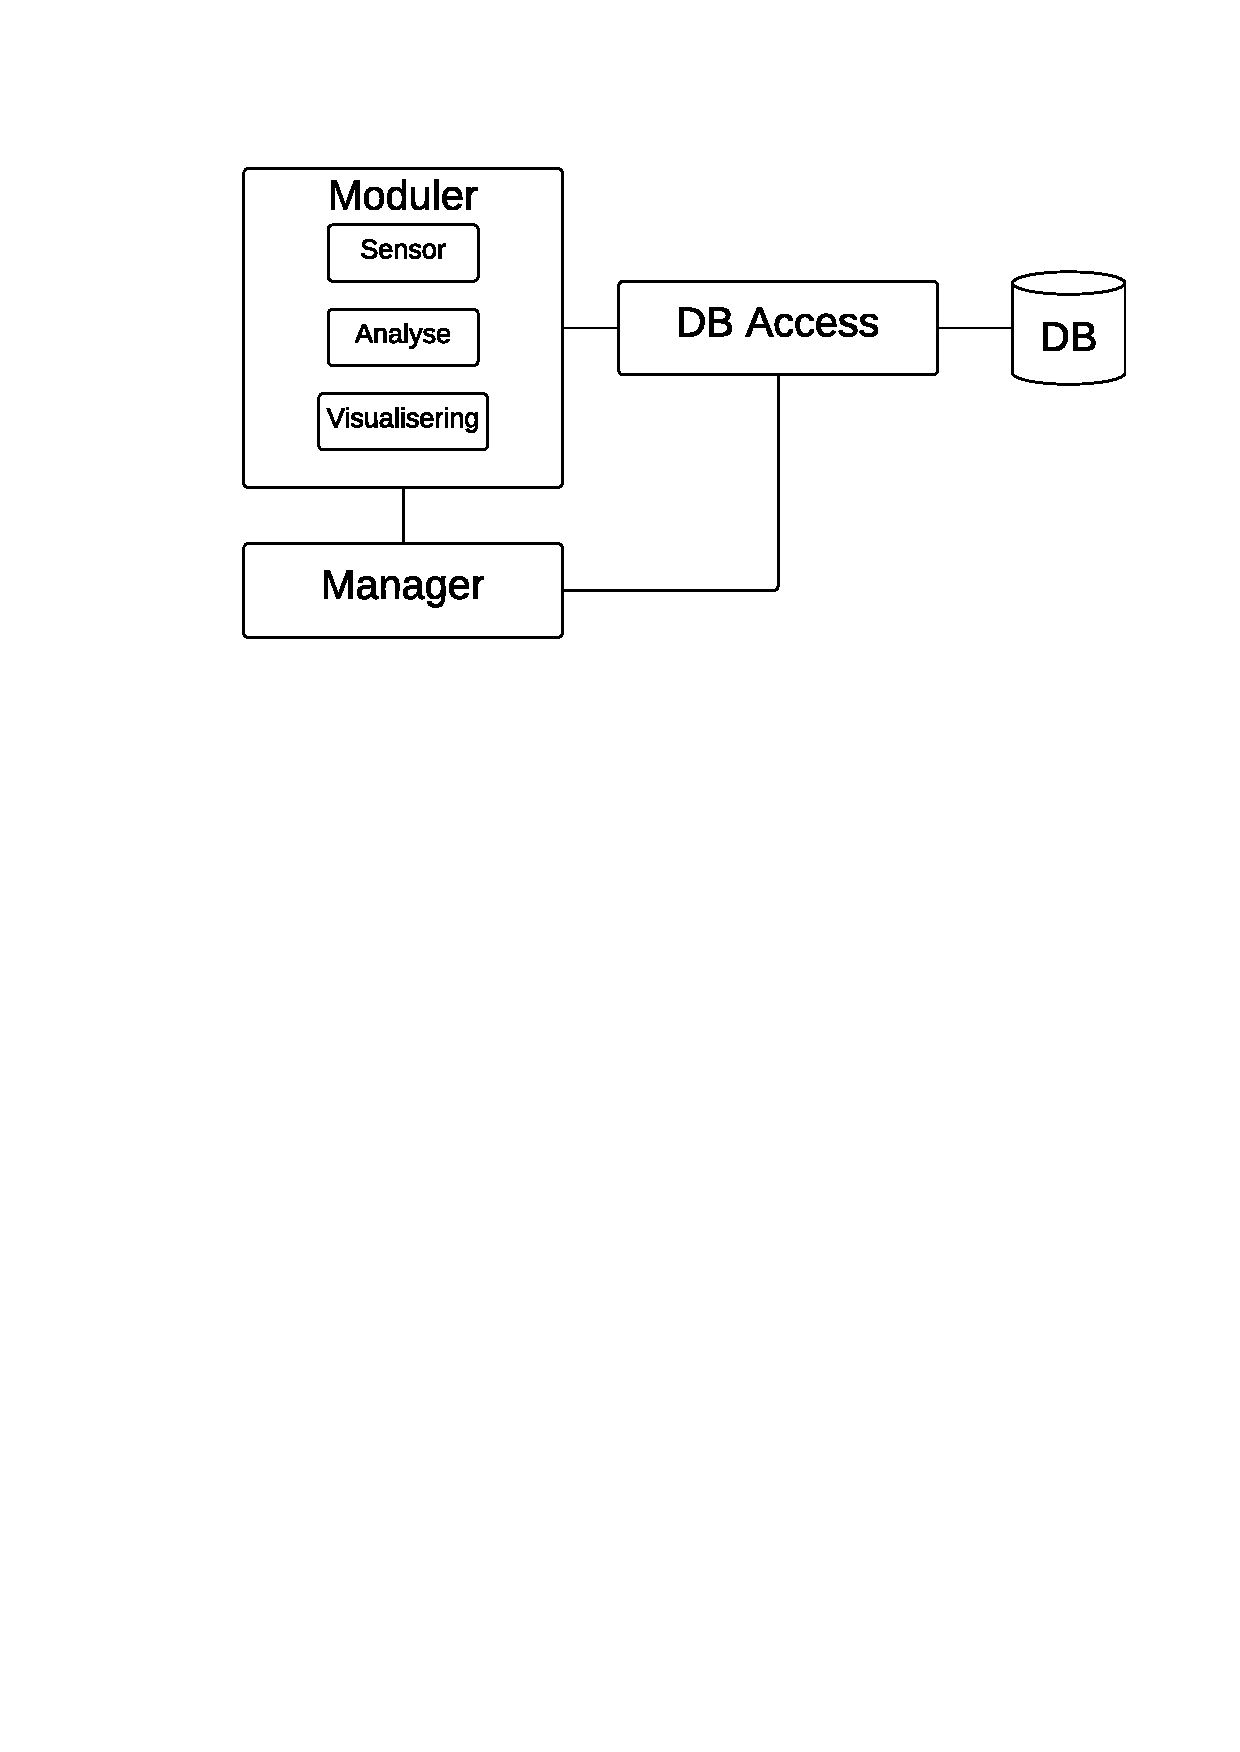
\includegraphics[scale=0.5, trim = 1cm 17.5cm 1cm 1cm, clip]{../grafik/ArkitekturLucidChart}
	\caption{Systemets arkitektur}
  \label{arkitektur_udkast_1}
\end{figure}
\end{frame}

\begin{frame}
\frametitle{Manager}
\begin{itemize}
\item Central kontrol enhed
\item Del brugeren interagerer med
\item Kontrollerer hvilke moduler der skal køre
\item Finder moduler på telefonen
\end{itemize}
\end{frame}

\begin{frame}
\frametitle{Kriterier}
Kriterierne dækkes af følgende elementer i arkitekturen:
\begin{itemize}
\item Modulær $\rightarrow$ Moduler
\item Fleksibel $\rightarrow$ Manager
\item Kombinerbar $\rightarrow$ Moduler
\item Kommunikativ $\rightarrow$ DB Access/DB
\end{itemize}
\end{frame}

\begin{frame}
\frametitle{Vedligeholdelse}
Ny viden
\begin{itemize}
\item Tilføje/forbedre modul(er)
\end{itemize}

\end{frame}

\begin{frame}
\frametitle{Nyt Modul}
At lave et nyt modul kræver
\begin{itemize}
\item Service
\item Modul definition.
\end{itemize}
\end{frame}

